\documentclass[11pt,a4paper]{article}
\usepackage[margin=2.5cm]{geometry}
\usepackage{graphicx}
\usepackage{enumitem}
\usepackage[svgnames]{xcolor}
\usepackage[most]{tcolorbox}
\usepackage[hidelinks]{hyperref} % o usar colorlinks como se explicó antes
\usepackage{listings}
\usepackage[spanish]{babel}
\usepackage{changepage}
\usepackage{enumitem}
\usepackage{capt-of}

\lstset{
	language=C, % Lenguaje: C
	basicstyle=\ttfamily\small, % Fuente monoespaciada, tamaño pequeño
	keywordstyle=\color{Blue}\bfseries, % Palabras clave en azul y negrita
	stringstyle=\color{Red}, % Cadenas en rojo
	commentstyle=\color{Green}, % Comentarios en verde
	numbers=left, % Numeración de líneas a la izquierda
	numberstyle=\tiny\color{Gray}, % Estilo de números de línea
	stepnumber=1, % Numerar cada línea
	numbersep=5pt, % Distancia de números al código
	showspaces=false, % No mostrar espacios
	showstringspaces=false, % No marcar espacios en cadenas
	frame=single, % Marco alrededor del código
	tabsize=4, % Tamaño de tabulación
	breaklines=true, % Romper líneas largas
	breakatwhitespace=true, % Romper solo en espacios
}

\begin{document}
	\begin{titlepage}
		\begin{center}
			\begin{figure}
				\centering
				
\includegraphics[scale=0.2]{US-marca-principal.png}
			\end{figure}
			{\large \textbf{Escuela Técnica Superior de Ingeniería Informática}}
			\vspace{2mm}\\
			{Ingeniería Informática. Ingeniería de Computadores.}
			\vspace{60mm}\\
			\begin{center}
				{\huge \textbf{MEMORIA PRÁCTICA \uppercase\expandafter{\romannumeral 2\relax}}}\\[2mm]
				{Asignatura: Sistemas Empotrados y de Tiempo Real I}\\
				{Profesor: Gabriel Jiménez Moreno}
			\end{center}
			\vfill
			{Alumno: Álvaro José Gullón Vega}
		\end{center}
	\end{titlepage}
	\pagebreak
	\tableofcontents
	\pagebreak
	
	\section{Objetivos}
	\large{
		En esta segunda práctica distinguimos dos objetivos:
		
		\subsection{Académico}
		Los objetivo académicos en este caso, constan de estudiar y entender el funcionamiento de los Displays LCD tradicionales que se usan con los microcontroladores, conocer los aspectos más básicos de la placa de desarrollo de la asignatura y entender las diferencias entre las diversas librerías que proporcionan los fabricantes para el manejo de los periféricos en los microcontroladores tipo Cortex.
		
		\subsection{Práctico}
		Para conseguir estos objetivos académicos, se han propuestos estos objetivos prácticos:
		\begin{itemize}
		\item Mandar texto a cualquier posición en un display tipo HD44780.
		\item Definir un nuevo dibujo en la memoria del Display y visualizarlo en pantalla
		\item Manejar los LEDs y el botón de la placa al igual que se hizo en la práctica 1.
		correspondientes a ese pin y conectadas a VCC o a GND.
		\item Sustituir en la librería del display LCD, que se proporciona en esta práctica, las llamadas a las funciones GPIO LL por funciones equivalentes GPIO HAL.
		\end{itemize}
	}
	
	\section{Introducción}
	\large{
		Como hemos mencionado en los objetivos, esta segunda práctica nos acercará a conocer los Display LCD al igual que nos ofrecerá una primera toma de contacto con la placa que usaremos en la asignatura.\\
		
		Las interfaces visuales más primitivas están basadas en LEDs, un ejemplo de ellos los displays de siete segmentos, los que si agrupamos varios de ellos podemos componer una interfaz visual más completa con un problema que es la cantidad de pines que se requieren para su control. Por otra parte contamos con los displays LCD u OLED, dos tecnologías que han evolucionado mucho los últimos años con las que se construyen un gran número de dispositivos de visualización destinados a su uso con microcontroladores.
		
		Nosotros, en SETR1, nos vamos a centrar en el uso de displays más modestos y primitivos que suelen disponer de dos tipos de interfaces:
		\begin{itemize}
			\item \textbf{Paralela:} Consiste en un bus de ocho bits \textit{(D0-D7)} y tres líneas de control \textit{(RS, E, R/W)}. El bus de datos es bidireccional de forma que podemos escribir en el display o podemos leer de él como por el ejemplo el bit de estado.
			
			\begin{center}
				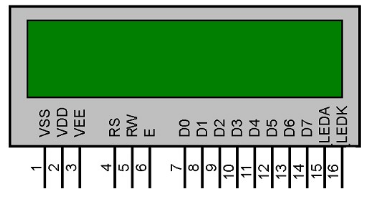
\includegraphics[width=0.6\textwidth]{pinout-display.png}
				\captionof{figure}{Pinout típico del Display LCD.}
			\end{center}
			
			\item \textbf{Serie síncrona:} Usan normalmente puertos \textit{I2C} o \textit{SPI}. Se utilizan dos o tres líneas de conexión con el microcontrolador.
		\end{itemize}
		
		El circuito de control es el cerebro del display, por un lado tiene los pines que sirven de interfaz con el usuario y por otra controla la pantalla de visualización. Casi siempre suelen tener una memoria RAM, excepto los más sofisticados que incluyen de dos en adelante para por ejemplo en la GameBoy organizarlas como memoria principal, memoria de background, memoria de tejas, etc...\\
		
		La pantalla donde se muestra la información en ocasiones su tamaño es independiente de la capacidad de direccionamiento de la memoria del controlador, y no tienen por qué coincidir. 
	}
	
	\section{Desarrollo de la práctica}
	\subsection{Fase 1: Usar el display HD44780 y empezar a manejar la placa de la asignatura.}
	
	
	\subsection{Fase 2: Repetir la Fase 2 y 4 de la práctica 1 con la nueva placa.}
	
	\subsection{Fase 3: Repetir la fase 1 de esta práctica, pero usando librerías HAL.}

	\section{Contestación de preguntas}
	
	\section{Conclusiones}

\end{document}